% CSE 521S Final Report
% A Parking Guidance and Information System for TinyOS
% By Matthew Lindsay, Patrick McBryde, Michael Schultz

\documentclass{acm_proc}
\usepackage{hyperref}
\usepackage{url}
\usepackage{graphicx}

\begin{document}

\title{A Parking Guidance and Information System for TinyOS}
\subtitle{CSE 521S Final Report}

\numberofauthors{3}
\author{
\alignauthor Matthew Lindsay\\
% 2nd. author
\alignauthor Patrick McBryde\\
% 3rd. author
\alignauthor Michael Schultz\\
\and
\affaddr{Washington University in Saint Louis}\\
}

\maketitle

\begin{abstract}
``Intelligent Transportation Systems'' (ITS) are a mix of systems that
gather various data metrics from transportation areas (parking lots,
streets, alleyways, etc.), aggregate this data together, and present
coherent information to the end-users of the system.
Orchestrating such a system presents several challenges at each level.
How do you gather the data and at what granularity?
Where does the data go once gathered and can it be useful to anyone?
If it can be useful, how can it be presented to end-users to provide
accurate and simple-to-interpret content?
This paper presents and explains our decisions in developing a ``Parking
Guidance and Information'' (PGI) system for TinyOS.
\end{abstract}

\section{Introduction}

Driving to new destinations always brings some level of stress and
uncertainty.
Where am I going, what do the roads and intersections look like, what side
of the road is the place on, where do I park?
These are all questions that dart through the brain when beginning to think
about going some place new.
Luckily, maps bring us the answer or at least a partial answer to some of
those questions.
In the past decade there has been huge growth of web-based mapping
technology to help answer these questions even more fully.
For example, Google Maps allows you to get directions from point A to point
B, and in the past 5 years has introduced Street
View~\cite{vincent:streetview} to their interface.
Street View allows a user to view the roads they will be travelling on from
an in-car perspective.
This removes much of the uncertainty when driving, leading to less
confusion and a better experience (and potentially fewer accidents).

However, there is still that can be done.
Even after you've arrived at your destination you must find where to park.
This can also be quite a hassle, as you are unfamiliar with the area and
during peak hours there may not be a parking space in near proximity.
To help in this matter, Parking Guidance and Information Systems (PGIS)
allow drivers to quickly evaluate where best to go to find parking
efficiently~\cite{sakai:pgi-toyota}.
Traditional PGI Systems simply count the number of cars that enter and exit
a designated area and display the number of spots available in that area to
the driver.
These systems are imprecise, costly, and can't be integrated with other
technologies.

This paper presents our experiences building a parking guidance and
information system using the TelosB/TinyOS platform.
By using motes, it opens the possibility of deploying a single sensor for
each available parking space allowing for much more detailed information
about a parking lot as a whole.
Moreover, with proper sheltering, these sensors can be mounted on the
surface of a parking lot instead of cutting into the lot and installing an
inductive loop to detect vehicle presence.
We also take advantage of the wireless multi-hop routing abilities of
TinyOS-based motes to avoid wiring and enable a heterogeneous mix of
sensors to keep track of parking spot availability and usage data.
Combining these aspects gives a system that can be more precise, lower
cost, and more easily integrated with future technologies.

The remainder of this paper is as follows.
Section~\ref{sec:goals} defines the goals of this project more fully.
Section~\ref{sec:design} presents and explains the high-level architecture
of our PGI System and details the hardware and software we depend on.
Section~\ref{sec:implementation} discusses the backend implementation of
our system to aggregate and store the data we collect from the sensors.
Section~\ref{sec:experiment} talks about how we convinced ourselves that
the system worked correctly and, if we have more resources, could scale up
as needed.
Sections~\ref{sec:related} and~\ref{sec:lessons} give an overview of
related works and lessons we learned during this project.
Finally, Section~\ref{sec:conclusions} concludes this paper with a
discussion of potential future work for this project.

\section{Goals}\label{sec:goals}

What are the goals for this project, what we set out to do (in detail).

% Answer the questions in the abstract:
% - How do you gather the data and at what granularity
% - Where does the data go once gathered and can it be useful to anyone
% - How can it be presented to end-users to provide accurate and
%   simple-to-interpret content?

% from proposal
To achieve these goals, we intend to use the Tmote Sky/TelosB mote platform
which have an expansion connector that allows external sensors to be
connected.
To reduce installation costs, we will use a multi-hop routing protocol
(likely
the collection tree protocol) to communicate data from a sensor to the base
station.
This allows for a large number of sensors to be deployed with little effort
or
physical infrastructure to be in place.
Finally, once the data is aggregated at a central location it must be
displayed
to the end user in an easy to read/interpret interface.
This is important because the vehicle operator needs to have a quick,
intuitive
knowledge of where to go, so they don't cause physical congestion.
We also wish to monitor the duration of parking space use, to allow a
parking
attendant to be notified when a person has overused their space.
% end from proposal

\section{Design}\label{sec:design}

\begin{figure}
    \begin{center}
		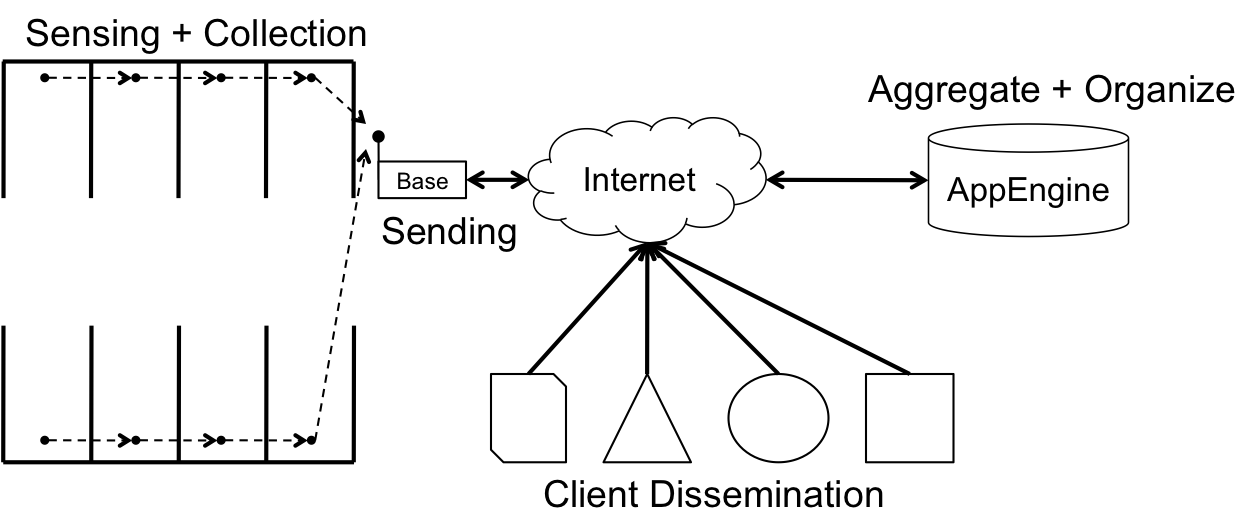
\includegraphics[width=\columnwidth]{figures/high-level}
	\end{center}
	\caption{High-level view of our PGI System. A base station at the lot
	sends data over the Internet to our aggregator, which end-users can
	query.}
	\label{fig:high-level}
\end{figure}

Figure~\ref{fig:high-level} shows a high-level view of the infrastructure
of our PGI System.
Our system begins with a parking lot (left side of
Figure~\ref{fig:high-level}), each space in this lot is equipped with a
sensor built on the TelosB/TinyOS platform.
Data is collected at a per-lot base station, which then sends the data over
the Internet to our backend.
When our backend receives the data it updates and logs the changes to the
data store and organizes the lot information.
Once the data is stored, clients are able to query the backend and get
up-to-date information about a specific lot and lots in the vicinity.

Building this system requires a fair amount of hardware and software
knowledge and is described below.

\subsection{Hardware}

This should cover the physical hardware we used in building this.
Including (but not limited to):

- TelosB motes (listing any relevant specifications, why we used TelosB
 and not something else) \cite{xbow:telosb-datasheet}.

- External sensor we used, specifications for that, more detail than
 TelosB since the reader will be less familiar with it, why we used that.

At least one pictures of the telosb, the sensors, or the telosb with sensor
attached.

% from proposal
We would like 6 TelosB/Tmote Sky sensors (2 for sensor testing and 4 for
network
development to build a non-trivial routing topology).
It would also be interesting to use a Mica family board with the MTS310CA
(magnetometer) sensor board, to test vehicle detection with a magnetometer,
though not strictly required as we can find other sensors to use.
Alternatively, if we can interface a magnetometer with the TelosB/Tmote Sky
mote board that could be used instead of a Mica family board.
% end from proposal

\subsection{Software}

Yup we had software.

A paragraph or two about TinyOS and building whatever we used there
(interfaces, interaction with other sensors and base
station, CTP)~\cite{tep119:collection}.

A paragraph about the base station software and what it does.

A paragraph laying out what Google AppEngine is, why we chose it, and what
it does for us.

A paragraph or two describing the AE backend and frontend(s).

\section{Implementation}\label{sec:implementation}

More detailed description of the underlying implementation (packet formats
in the network, sending data to AppEngine, specific technology used on
backend, any frontend stuff).

% from proposal
The major components of this project are building and developing the
sensing
devices, writing and testing the networking and communications
software to handle data delivery, and creating a friendly front end to
present
and track the information as needed.
If we discover any of these components are significantly easier than
others, it
is easy to combine forces to develop new/better methods for any of them.
We also have an interest in discovering more specific information of
existing
systems and getting up-to-date in the area of intelligent transportation
systems.
% end from proposal

\section{Experiment}\label{sec:experiment}

Paragraph about experiments that show our system works.

\section{Related Work}\label{sec:related}

We are aware of two systems that target per-spot granularity.
The first, Signal-Park, uses sonar sensors above each parking spot to
detect the presence of a vehicle~\cite{pgi:signal-park}.
Approximately three times per second, the sensor is queried to determine
vehicle presences and updates a central computer.
This system uses serial lines to connect each sensor with the central
computer, leading to more costly deploy.
It also appears to be limited to the parking lot that it is deployed in and
lacks the ability to aggregate the information for others to benefit.
It would certainly be possible to improve the connectivity of this system
to integrate with our back-end aggregation system to take advantage of
existing installations.

The other system, Streetline, is a startup in the San Francisco area
that similarly uses a wireless mesh network to link all the sensors
together~\cite{pgi:streetline}.
The Streetline system has recently (Summer 2010) begun to roll out sensors
and upgraded meters for select areas in the San Francisco
area~\cite{wired:streetline, sfpark}.
This system uses surface (and sub-surface) sensor mounts that contain a
wireless transmitter and a magnetometer for vehicle detection.
Status is sent to a central aggregation server where users can see the
status of street parking via their web browser, text message, or smart
phone; it also allows municipal workers to identify vehicles that have not
paid fully.
Presuming the Streetline trial is successful and the system expands, our
system and their system should be able to integrate with little effort and
could be seen as competitors.
We view this a positive, as it demonstrates that our project is a useful
idea with potential buyers available.

\section{Lessons Learned}\label{sec:lessons}

Anything we would have done differently if we were to pursue this project
in more detail again.

\section{Conclusions and Future Work}\label{sec:conclusions}

Conclusions from this project.

% \section{References}
\bibliographystyle{abbrv}
\bibliography{report}

\end{document}
